\documentclass[a4paper]{tufte-handout}

\usepackage{/Users/paulallen/OU/Maths/style}

    \usetikzlibrary{shapes.geometric}
  
\begin{document}
\tma{01}

%%%%%%%%%%Question one
\begin{question}

\qpart
$-\frac{3}{7}$ is a rational number.\\
\bigskip
$\sqrt{2}$ is an irrational number.\\
\bigskip
$-6$ is an integer.\\

\vspace{1.5cm}

\qpart
\qsubpart
\[10-(2\times+3\times2^2+1)=-9\]
\hfill i. (B)\\
\qsubpart
\[10-3\times2+3\times(2^2+1)=19\]
\hfill ii. (C)\\
\qsubpart
\[10-3\times(2+3\times2^2)+1=-31\]
\hfill iii. (A)

\vspace{1.5cm}

\qpart 
Given; $0.0476$

\qsubpart
\[0.05\]\hfill (to 2 d.p)\\
\qsubpart
\[0.048\]\hfill (to 2 s.f)

\pagebreak

\qpart
When:
\[a=-3 \qquad b=-5\]

\begin{align*}
\frac{1-a^2}{b} &= \frac{8}{5}\\[8pt]
\frac{1-(-3)^2}{-5} &= \frac{8}{5}\\[8pt]
\frac{1-9}{-5} &= \frac{8}{5}\\[8pt]
\frac{8}{5} &= \frac{8}{5}
\end{align*}
\hfill \text{As required}

\vspace{1.5cm}

\qpart

\begin{tabular}{cccccc}
$558$&$=$&\textcolor{red}{$2^2$}&$3$&$7^2$& \\
$616$&$=$&$2^3$&&\textcolor{red}{$7$}&$11$
\end{tabular}

The HCF is $2^2\times7=28$
\hfill As required


\end{question}

%%%%%%%%%%%Question two
\begin{question}

\qpart
Simplify the given expressions.

\qsubpart
Given expression:
	\[v \times vw^2 \times v^2w^3\]

\bigskip

First, multiply the first two terms:
	\[v^2w^2 \times v^2w^3\]

\bigskip

Then, multiply the result with the remaining terms:
	\[v^2w^2 \times v^2w^3\]

\bigskip

Final answer:
	\[v^4w^5\]
	
\vspace{1.5cm}
	
\qsubpart
Given expression:
	\[-2xy + (-3x \times 2y^2) - (-xy)\]
	
\bigskip	
	
Distribute the brackets
	\[2xy -6xy^2 + xy\]
	
\bigskip	
	
Collect like terms;
	\[xy -6xy^2\]
	
\bigskip
	
Factorise for the final answer; 
	\[xy(1-6y)\]

\pagebreak

\qpart
Expand and simplify these expressions;
	
\qsubpart
Given expression;
\[7(e-f) -2(e+f)\]

\bigskip

Distribute the brackets;
	\[7e - 7f -2e -2f\]
	
\bigskip	
	
Collect like terms:
	\[7e -2e -7f -2f\]
	
\bigskip
	
Final answer:
	\[5e -9f\]
	
\vspace{1.5cm}
	
\qsubpart
Given expression
	\[(x-2)(x+2) + x(x-3) \]
	
\bigskip	
	
Distribute first 2 sets of brackets
	\[x^2 -4 + x(x-3)\]
	
\bigskip	
	
Distribute final set of brackets:
	\[x^2 -4 +x^2 -3x\]
	
\bigskip	
	
Collect like terms;
	\[x^2 + x^2 -3x -4\]
	
\bigskip
	
Final answer:
	\[2x^2 -3x -4\]
	
\pagebreak
	
\qsubpart
Given expression
	\[(2m +3n)^2 = (2m +3n)(2m +3n)\]
	
\bigskip	
	
Multiply out the brackets
	\[4m^2 +6mn +6mn +3n^2\]
	
\bigskip
	
Collect like terms, final answer;
	\[3m^2 +3n^2 +12nm\]
	
\vspace{1.5cm}

\end{question}
%%%%%%%%%%%%Question three	
\begin{question}

\qpart
Factorise the following expressions;

\qsubpart
Given expression:
	\[3pq -21pr\]
	
\bigskip	
	
Factor out the HCF, $3$:
	\[3(pq -7pr)\]
	
\bigskip	
	
Factor out the common factor, $p$:
	\[3p(q -7r)\]
	
\pagebreak
	
\qsubpart
Given expression:
	\[\frac{2}{5}y^2z + \frac{1}{2}y^3z^4\]
	
\bigskip	
	
Multiply by the LMC, $10$:
	\[\frac{20}{5}y^2z + \frac{10}{2}y^3z^4\]

\bigskip
	
Distribute the terms;
	\[4y^2z +5y^3z^4\]
	
\bigskip	
	
Factor out the common factor, $y^2$:
	\[y^2(4z + 5yz^4)\]
	
\bigskip	
	
Factor out the common factor, $z$, final answer:
	\[y^2z(4 +5yz^3)\]

\vspace{1.5cm}
	
\qpart
Simply the following algebraic fractions

\qsubpart
Given fraction:
	\[\frac{24s^5t}{18s^2t^3}\]
	
\bigskip
	
Divide by $6$:
	\[\frac{4s^5t}{3s^2t^3}\]
	
\bigskip	
	
Divide by $s^2$:
	\[\frac{4s^3t}{3t^3}\] 
	
\bigskip
	
Divide by $t$, final answer:
	\[\frac{4s^3}{3t^2}\]
\hfill Where $s, t \neq 0$.

\pagebreak

\qsubpart
Given fraction:
	\[\frac{2v^3+v^2}{8v+4}\]
	
\bigskip
	
Factor out $4$ from $8v+4$:
	\[\frac{2v^3+v^2}{4(2v+1)}\]
	
\bigskip	
	
Factor out $v^2$ from $2v^3+v^2$:
	\[\frac{v^2(2v+1)}{4(2v+1)}\]
	
\bigskip	
	
Final answer:
	\[\frac{v^2}{4}\]
\hfill Where $v \neq\frac{-1}{2}$.

\vspace{1.5cm}
	
\qpart
Write the following as a single fraction:
	\[\frac{2}{c}-\frac{3}{cd}+\frac{1}{d}\]
	
Write all fractions with the common denominator $cd$:
	\[\frac{2d}{cd}-\frac{3}{cd}+\frac{c}{cd}\]
	
Final answer:
	\[\frac{c+2d-3}{cd}\]
\hfill Where $c, d \neq 0$.

\pagebreak

\qpart
Simplify the following expression:
\[\biggl(\frac{2b}{a}\biggl)\biggl/\biggl(\frac{b^3-2ab^2}{4a^3-2a^2b}\biggl)\]

Multiply by the reciprocal:
	\[\frac{2b}{a}\times\frac{4a^3-2a^2b}{b^3-2ab^2}\]
	
\bigskip	

	\[\frac{8a^3b-4a^2b^2}{ab^3-2a^2b^2}\]
	
Factor out $-4a^2$ from $4a^3-2a^2b$;
	\[\frac{-4a^2(b^2-2ab)}{ab^3-2a^2b^2}\]
	
\bigskip	
	
Factor out $ab$ from $ab^3-2a^2b^2$
	\[\frac{-4a^2(b^2-2ab)}{ab(b^2-2ab)}\]
	
\bigskip
	
Cancel terms:
	\[\frac{-4a^2}{ab}\]
	
\bigskip	
	
Final answer;
	\[\frac{-4a}{b}\]
\hfill Where $a, b \neq 0$ and $2a \neq b$.

\end{question}

%%%%%%%%Question four
\begin{question}

\qpart
Show that:
\begin{align*}
\sqrt{7}(\sqrt{5}+\sqrt{3})-\sqrt{80}&=\sqrt{35}+\sqrt{21}-4\sqrt{4}\\[5pt]
 &= \sqrt{7}\times\sqrt{5}+\sqrt{7}\times\sqrt{3} -\sqrt{80}\\[5pt]
 &= \sqrt{7\times5} +\sqrt{7\times3} -\sqrt{80}\\[5pt]
 &= \sqrt{35} +\sqrt{21} -\sqrt{16\times5}\\[5pt]
 &= \sqrt{35} +\sqrt{21} -\sqrt{16}\times\sqrt{5}\\[5pt]
 &= \sqrt{35} +\sqrt{21} -4\sqrt{5}\\
\end{align*}
\hfill As required

\qpart
Rationalise the denominator;
	\[\frac{\sqrt{200}}{\sqrt{8}+\sqrt{3}}\]

Multiply by the conjugate radical;
	\[\frac{\sqrt{200}}{\sqrt{8}+\sqrt{3}}\times\frac{\sqrt{8}-\sqrt{3}}{\sqrt{8}-\sqrt{3}}\]
\bigskip
	\[\frac{\sqrt{200}\times\sqrt{8}-\sqrt{200}\times\sqrt{3}}{(\sqrt{8}-\sqrt{3})(\sqrt{8}-\sqrt{3})}\]
	
\bigskip

Simply:
	\[\frac{\sqrt{1600}-\sqrt{600}}{\sqrt{8}\sqrt{8}-\sqrt{8}\sqrt{3}+\sqrt{3}\sqrt{8}-\sqrt{3}\sqrt{3}}\]

\bigskip
	\[\frac{40-\sqrt{100}\times\sqrt{6}}{8-3}\]
\bigskip
	\[\frac{40-10\sqrt{6}}{5}\]
Final answer:
	\[8-2\sqrt{6}\]

\pagebreak

\qpart
\begin{flalign*}
\text{Using the index law, } (ab)^{n} = a^{n} b^{n}\\
    \frac{(3b^{2}c^{-1})^{3}}{bc^{2}} &= \frac{3^{3}(b^{2})^{3}(c^{-1})^{3}}{bc^{2}} \\[8pt]
\text{Then, using the index law, } (a^m)^n = a^{mn}\\
    &= \frac{3^{3} b^{6} c^{-3}}{bc^{2}} \\[8pt]
\text{Next, using the index law } a^{-n} = \frac{1}{a^n} \\
    &= \frac{3^{3} b^{6} b^{-1}}{c^{3} c^{2}} \\[8pt]
\text{Finally, using the index law } a^{m} a^{n} = a^{m+n}\\
    &= \frac{27b^{5}}{c^{5}}
\end{flalign*}

\vspace{1.5cm}

\qpart
Simplify the following expression

Given expression:
	\[\frac{\sqrt[4]{(256x^3)}x^{\frac{-1}{2}}}{(64x^{4})^{\frac{1}{5}}}\]
	
Rewrite the roots in Index Form:
	\[\frac{(256x^{3})^{\frac{1}{4}}x^{\frac{-1}{2}}}{64^{\frac{1}{5}}(x^{4})^{\frac{1}{5}}}\]

Distribute the exponents:
	\[\frac{256^{\frac{1}{4}}(x^{3})^{\frac{1}{4}}x^{\frac{-1}{2}}}{64^{\frac{1}{5}}(x^{4})^{\frac{1}{5}}}\]
	
Simplify each power:
	\[\frac{256^{\frac{1}{4}}x^{\frac{3}{4}}x^{\frac{-1}{2}}}{64^{\frac{1}{5}}x^{\frac{4}{5}}}\]
	
Combine like terms in the numerator:
	\[\frac{256^{\frac{1}{4}}x^{\frac{1}{4}}}{64^{\frac{1}{5}}x^{\frac{4}{5}}}\]
	
Simplify the fraction of exponents on x:
	\[\frac{256^{\frac{1}{4}}x^{\frac{-11}{20}}}{64^{\frac{1}{5}}}\]

Rewrite the denominator as a radical: 
	\[\frac{256^{\frac{1}{4}}x^{\frac{-11}{20}}}{\sqrt[5]{64}}\]

Evaluate the radicals for 256 and 64:
	\[\frac{4x^{\frac{-11}{20}}}{\sqrt[5]{32}\sqrt[5]{2}}\]
	
Further simplify the denominator:
	\[\frac{4x^{\frac{-11}{20}}}{2\sqrt[5]{2}}\]
	
Combine exponents on 2:
	\[\frac{2x^{\frac{-11}{20}}}{2^{\frac{1}{5}}}\]

Final answer:
	\[\frac{2^{\frac{4}{5}}}{x^{\frac{11}{20}}}\]

\end{question}

%%%%%%%% Question five
\begin{question}

\qpart
   
\begin{align*}
7x + 6y &= 45\\[8pt]
\shortintertext{Substitute: }
7(3) + 6(4) &= 45\\[8pt]
\shortintertext{Evaluate: }
21 + 24 &= 45 \snote{as required}
 \end{align*}

\qpart
Solve:

\begin{flalign*}
\shortintertext{Given equation: }
2(x-3)&=4-\frac{x}{2}\\[8pt]
\shortintertext{Multiply out the brackets: }
2x-6&=4-\frac{x}{2}\\[8pt]
\shortintertext{Multiply by $2$: }
4x-12&=8-x\\[8pt]
\shortintertext{Collect like terms: }
4x-x&=8+12\\[8pt]
\shortintertext{Evaluate: }
5x&=20\\[8pt]
\shortintertext{Final answer: }
x&=4
\end{flalign*}


\qpart
Solve:
	
\begin{align*}
\frac{4}{x+2}+\frac{5}{2-3x}&=0\\[8pt]
\shortintertext{Given equation: }
\frac{4}{x+2}+\frac{5}{2-3x}&=0\\[8pt]
\shortintertext{Cross multiply: }
4(2-3x)+5(x+2)&=0\\[8pt]
\shortintertext{Distribute the brackets: }
8-12x+5x+10&=0\\[8pt]
\shortintertext{Collect like terms: }
10+8&=12x-5\\[8pt]
\shortintertext{Evaluate: }
18&=7x\\[8pt]
\shortintertext{Final answer: }
x&=\frac{18}{7}\\[8pt] \snote{$\biggl(x\neq-2$  and  $x\neq\frac{2}{3}\biggl)$}
\end{align*}

\qpart
Make $y$ the subject

Given equation
	\[xy+z=\frac{1}{z}-yz\]
	
\begin{flalign*}
xy+z=&\frac{1}{z}-yz\\[8pt]
\shortintertext{Multiply by $z$: }
xyz+z^{2}=&1-yz^{2}\\[8pt]
\shortintertext{Collect like terms: }
xyz+yz^{2}=&1-z^{2}
\shortintertext{Factor out $y$: }
y(xz+z^{2})=&1-z^{2}
\shortintertext{Divide by $(xz+z^{2})$: }
y=&\frac{1-z^{2}}{xz+z^{2}}
\shortintertext{Final answer: }
y=&\frac{1-z^{2}}{z(x+z)}
\end{flalign*}

\end{question}
 
 %%%%%%%%%%%%Question six
\begin{question}

\qpart
\begin{itemize}
\item The given solution makes no reference to which calculation belongs to which design. 
\item The calculations do not indicate why each equation is used.
\item The solutions do not contain units.
\item The question asks for the answer to be given to the nearest penny, and neither answer does.
\item The use of $*$ instead of $\times$ is inappropriate.  
\end{itemize}

\vspace{2cm}

\qpart
\textbf{Design one}
The first design option is a trapezium-shaped turf lawn, with parallel sides of \SI{4}{\metre} and \SI{7}{\meter} and a perpendicular height of \SI{6}{\metre}.

\begin{tikzpicture}
  \node [trapezium, trapezium angle=60, minimum width=50mm, draw, thick, label=above:$4m$, label=below:$7m$] {};
  \draw[>=triangle 45, <->] (0,-1.2) -- (0,1.2);
  \node[left] {$6m$} (0,0);
\end{tikzpicture}

The area of a trapezium is given by the formula; \[\frac{1}{2}(a+b)h\]

\begin{align*}
\shortintertext{Area of the lawn: }
\frac{1}{2}(a+b)h&=area\\[8pt]
\shortintertext{Substitute dimensions: }
\frac{1}{2}(4+7)6&=area\\[8pt]
\shortintertext{Total area}
area &=\frac{1}{2}(11)6\\[8pt]
area &=\frac{1}{2}(66)\\[8pt]
area &= \SI{33}{\metre\squared}\\
\end{align*}
 
 \pagebreak
 
The cost of turf is $\pounds5\unit{\per\metre\squared}$.

Therefore the total cost of the design would be \[\SI{33}{\metre\squared} \times \pounds5\unit{\per\metre\squared}=\pounds165.00\] 

\textbf{Design 2}
The second design is a circular lawn with a diameter of $\SI{7}{\metre}$, so a radius of \SI{3.5}{\metre}.

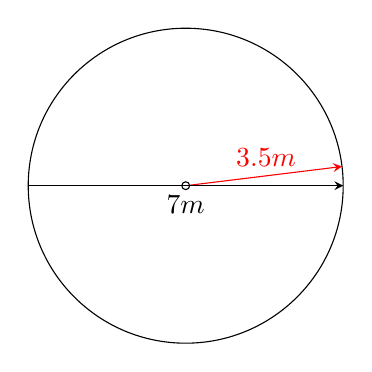
\begin{tikzpicture}
\draw (0,0) node[circle,draw,inner sep=1pt](o) {}
circle (2);
\draw[-stealth, red] (o) -- (7:2) node[midway,above]{$3.5m$};
\draw[-stealth] (0:-2) -- (0:2) node[midway,below]{$7m$};
\end{tikzpicture}

The area of a circle is given by the formula; \[\pi r^{2}\]

\begin{align*}
\shortintertext{Area of the lawn: }
\pi r^{2} &= area\\[8pt]
\shortintertext{Substitute dimensions: }
\pi \times 3.5^{2}&=area\\[8pt]
\shortintertext{Total area}
area &=\pi \times 12.25\\[8pt]
area &=12.25\pi\\[8pt]
area &= \SI{38.484}{\metre\squared}\ldots\\
\end{align*}

The area of turf needed would be $\frac{49}{4}\pi \unit{\metre\squared}$, approx $\SI{38.5}{\metre\squared}$. As we can only buy turf by the $\unit{\metre\squared}$ we would need to buy $\SI{39}{\metre\squared}$

The cost of turf is $\pounds5\unit{\per\metre\squared}$.

Therefore the total cost of the design would be \[\SI{39}{\metre\squared} \times \pounds5\unit{\per\metre\squared}=\pounds195.00\] 

\end{question}  

%%%%%%%%%%%%%Question seven
\begin{question}

PDF from Maxima included.

\includepdf[pages=-]{question_7.pdf}
\end{question}

%%%%%%%%%%%%%%Question eight
\begin{question}
\qpart

\vspace{4cm}

\qpart
\qsubpart
\begin{tabular}{|c|c|}
\hline
Task & score\\
Working with Bidmas&5\\ \hline
Rounding numbers&5\\ \hline
Algebraic substitution&4\\ \hline
Rearranging fractions&4\\ \hline
Multiplying out brackets&4\\ \hline
Factorising expressions&4\\ \hline
Simplifying algebraic expressions&5\\ \hline
Solving equations&5\\ \hline
Rearranging equations&5\\ \hline
\end{tabular}

\qsubpart
\begin{tabular}{|c|c|}
\hline
Task & Score\\
Working with coordinates&5\\ \hline
Sketching straight line graphs&5\\ \hline
Understanding gradients and intercepts&5\\ \hline
Parallel and perpendicular lines&5\\ \hline
Solving simultaneous equations&4\\ \hline
Factorising quadratics&4\\ \hline
Solving quadratics using different methods&4\\ \hline
Sketching quadratic equations&4\\ \hline
Solving real life problems involving quadratic equations&4\\ \hline
\end{tabular}

\end{question}


\end{document}
